
\documentclass[leqno,10pt]{article}
\usepackage{algorithm}
\usepackage[noend]{algpseudocode}
\usepackage{hyperref}
\usepackage[linewidth=1pt]{mdframed}
\usepackage{float}
\def\Z{\mathbb Z}
\def\Q{\mathbb{Q}}
\def\A{\mathbb{A}}

\makeatletter
\renewcommand{\ALG@name}{Algorytm}
\makeatother

\usepackage{amsmath}
\usepackage{float}
\usepackage{delta}
\usepackage{todonotes}
\usepackage{authblk}

\newcommand{\edge}{\mbox{\rotatebox[origin=c]{90}{\ddagger}}\xspace} 

\def\marg#1{\marginpar{\scriptsize\raggedright#1}}

\begin{document}

\wtyt{O pewnym modelu zawijania białek}


\waut{Marcin WIERZBIŃSKI$^{1,2}$, Karolina L. TKACZUK$^{2}$, Alessandro CRIMI$^{2}$}


\marg{[1] Student Wydziału Matematyki, Informatyki i Mechaniki, Uniwersytet Warszawski, [2] Sano Centrum Medycyny Obliczeniowej w Krakowie}

Aminokwasy to małe cząsteczki stanowiące główny budulec białka. 
Można o nich myśleć jak o koralikach nawleczonych na sznurek, a sposób ich ułożenia w przestrzeni
decyduje o funkcji białka w komórce oraz o tym jak oddziałuje ono z innymi
elementami komórki. Z tego względu struktura przestrzenna danego białka jest dla
badaczy bardzo pożądaną informacją m.in. w przypadku projektowania leków.

Istnieje wiele możliwości odtworzenia kształtu białka występującego w naturze.
Jedną z bardziej standardowych jest ,,hodowla'' cząsteczki w warunkach
laboratoryjnych, imitujących te naturalne. 
Jest to metoda bardzo czasochłonna i nie zawsze skuteczna, gdyż uchwycenie białka
nie zawsze bywa możliwe -- białko może okazać się niestabilne i rozpaść się przed odtworzeniem jego
kształtu.

Alternatywą dla opisanej wyżej metody jest tworzenie trójwymiarowych struktur ,,w krzemie'' (tj. przy
użyciu komputera) w oparciu o modele teoretyczne. Podstawą tych ostatnich są istniejące już struktury białek (wcześniej odtworzone eksperymentalnie i zebrane w bazie białek \href{www.rcsb.org}{\textit{Protein Data Bank}}). W ostatnich latach duże zainteresowanie mediów zyskał projekt AlphaFold (\href{https://alphafold.ebi.ac.uk}{alphafold.ebi.ac.uk}), który do przewidywania struktur białek wykorzystuje sztuczną inteligencje.

Jednym z najprostszych modeli
struktury przestrzennej białek jest model hydrofobowo-polarny (HP), 
w którym aminokwasy podzielone są na dwa typy: $H$
(aminokwas hydrofobowy) i $P$ (aminokwas hydrofilowy). Białko jest w nim reprezentowane przez zagięcie danej skończonej sekwencji $s \in\{H, P\}^{k}$ w kracie $L=\mathbb{Z}^{3}$ lub $L=\mathbb{Z}^2$.
\textit{Zagięcie} to przekształcenie różnowartościowe $\omega:\{1,\ldots,k\} \rightarrow L$, takie że sąsiednie liczby odpowiadają sąsiednim
punktom z kraty, tzn.
\begin{equation*}
		 \omega(i) \neq \omega(j)
		 \quad\textrm{oraz}\quad
		 |\omega(i)-\omega(i+1)|=1
		 \quad\textrm{dla }
     1 \leq i<j \leq k, 
\end{equation*}
przy czym $|p-q|$ to zwyczajna (euklidesowa) odległość między punktami
$p$ i $q$.
Poszukiwane jest zagięcie o najmniejszej \textit{energii}, zdefiniowanej jako
\begin{equation}\label{basic:eng}
E_{c}(s, \omega)=(-1)\cdot\sum_{1 \leq i<j \leq n} [s(i)=H]\cdot [s(j)=H]\cdot
[|\omega(i)-\omega(j)|=1],
\end{equation}
gdzie $[\cdot]$ jest \textit{nawiasem Iversona}, który przyjmuje wartość 1, gdy jego zawartość jest prawdziwa, a 0 w przeciwnym przypadku. Wartość $-E_{c}(s,\omega)$ jest zatem liczbą par sąsiadujących w kracie aminokwasów typu $H$. Czasem nie uwzględnia się w tej liczbie tych par, które sąsiadują już w samej sekwencji $s$. Jednak nie ma to oczywiście wpływu na problem odnajdywania zagięcia o minimalnej energii.


\marg{\vspace*{-3cm}
\begin{center}
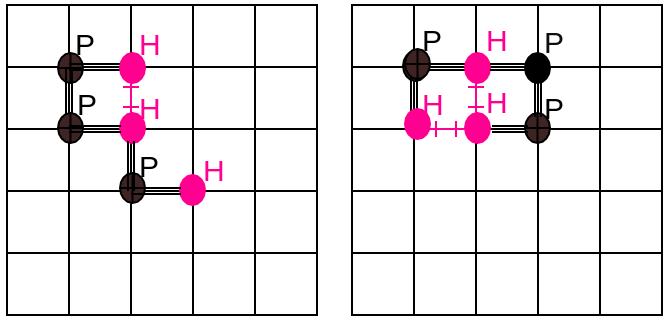
\includegraphics[width=4.8cm]{diagram3.png}
\end{center}
Przykłady zagięcia sekwencji $s={HPPHPH}$ w kracie $L=\mathbb{Z}^{2}$. Po
lewej stronie energia całkowita jest równa $-1$, a po prawej stronie $-2$.
Co więcej, zagięcie przedstawione po prawej stronie realizuje globalne minimum energii
całkowitej. 
}

Dla krótkich sekwencji aminokwasów (tzn. niewielkich wartości $k$) optymalne
zagięcie można odnaleźć, obliczając energię każdego możliwego zagięcia. W praktyce długości sekwencji mogą mieć od $50$ do ponad $1500$ aminokwasów. 
Liczba możliwych zagięć rośnie jednak bardzo szybko wraz ze wzrostem $k$! Umieszczonej na marginesie tabeli przedstawiono liczbę zagięć w kracie $\Z^3$ dla wybranych
wartości $k$.
\marg{
\begin{center}
\begin{tabular}{c|c}
$k$   &  liczba zagięć w $\Z^3$\\
\hline
1  & 6 \\
2  & 30 \\ 
3  & 150 \\
4  & 726 \\
5  & 3534 \\
10 & 8809878 \\
15 & $\sim 21{,}2\cdot 10^9$  \\
20 & $\sim 52 \cdot 10^{12}$ \\
\end{tabular}
\end{center}
}
Wartości podane dla $k=15,20$ są przybliżeniami obliczonymi przy użyciu metody
zaproponowanej przez Ariannę i Marshalla Rosenbluthów. Więcej o tej metodzie
można przeczytać w artykule Wojciecha Niemiro \textit{Monte Carlo, spacery i
polimery} w $\Delta_{15}^5$.

Sformułowany przez nas problem ma charakter obliczeniowy -- szukamy zagięcia $\omega$
minimalizującego energię zadaną przez \ref{basic:eng}. To zdanie może zostać przeformułowane w problem decyzyjny. 

\newpage
\begin{mdframed}
\textbf{Wejście}: Ustalona sekwencja $s \in \{H,P\}^{k}$, liczbę naturalna $m \in \mathbb{N}$.

\textbf{Pytanie:} Czy istnieje zawinięcie sekwencji $s \in \{H,P\}^{k}$ w kracie $
\mathbb{Z}^3$ o energii co najmniej $-m$? 
\end{mdframed}

Gdybyśmy znali szybki algorytm rozwiązujący powyższe zadanie, moglibyśmy
uruchamiać go dla coraz większych wartości $m$, by uzyskać informacje o
minimalnej energii zagięcia. Okazuje się jednak, że nasze decyzyjne zadanie jest
problemem NP-zupełnym. Potwierdzenie tej tezy można znaleźć w artykule \textit{Protein Folding in the Hydrohobic-Hydorplilic HP Model is NP-Complete} autorstwa Bonniego Bergera i Toma Leightona. 
W szczególności, nie istnieje szybki algorytm rozwiązujący nasz wyjściowy
problem odnajdywania optymalnego zawinięcia sekwencji aminokwasów. 

Do pokazania trudności problemu stosuje się ciekawy trik, który polega na wprowadzeniu
pewnego ogólniejszego problemu decyzyjnego, który jak się później okaże, jest
specjalnym przypadkiem problemu zawinięcia sekwencji. Rozpatruje się skończony ciąg $s$, zawierający $n^{3}$ typów $H$, które są idealnie włożone w kostkę rozmiaru $n \times n \times n$. Jeśli przypadek z taką kostką okaże się dosyć trudny, to oznacza, że nasz opisany problem także jest trudny. 

Przy poszukiwaniu optymalnego zagięcia, można czynić coś istotnie mądrzejszego niż konstruowanie losowego zagięcia. Jednym z podejść jest oznaczanie tras, którymi się już przechodziło i które nie dały interesującego zagięcia. Taki pomysł stosowany jest w algorytmie Monte Carlo Tree Search. Ten algorytm został wykorzystany m.in. w słynnej pracy Alpha Go. W listopadzie $2015$ roku jako pierwszy automat, Alpha Go pokonał zawodowego gracza w grę Go, Fan Hui,w pięciorundowym pojedynku na pełnej planszy w równej grze. AlphaGo był początkowo szkolony na archiwalnych grach, aby naśladować styl gry graczy, wykorzystując bazę danych zawierającą około $30$ milionów ruchów. 

W tej metodzie stosuję się tzw. drzewo możliwych ruchów. Drzewo jest przeszukiwane przy zastosowaniu odpowiedniej wagi dla wierzchołków, obliczonej na podstawie wcześniejszych symulacji ruchów. Każdą wagę wierzchołka w drzewie zwiększamy w kolejnych krokach, dbając o to, żeby przeszukiwanie drzewa było zbalansowane, tzn. staramy się dbać o różnorodność tras w drzewie możliwych ruchów. W szczegółach algorytm podzielony jest na 4 fazy: 
\begin{enumerate}
\item \textit{Wyboru}: rozpoczynamy od korzenia drzewa $R$ i wybieramy kolejne węzły potomne, aż do osiągnięcia węzła liściowego $L$. Korzeń to aktualny stan gry, a węzeł liściasty to każdy węzeł, który ma potencjalne dziecko, od którego nie rozpoczęto jeszcze symulacji (rozgrywki). Sposób wyboru węzłów podrzędnych pozwala na rozszerzanie drzewa możliwych ruchów w kierunku najbardziej obiecujących ruchów.
\item \textit{Rozszerzania}: jeśli $L$ nie kończy gry w sposób decydujący (np. wygrana/przegrana/remis) dla żadnego z graczy, należy utworzyć jeden (lub więcej) węzłów potomnych i wybrać węzeł $C$ z jednego z nich. Węzłami podrzędnymi są dowolne prawidłowe ruchy z pozycji w grze określonej przez $L$.
\item  \textit{Symulacji}: należy wykonać jedną losową rozgrywkę z węzła $C$. Ten krok jest czasem nazywany również playout lub rollout. Rozgrywka może być tak prosta, jak wybieranie jednakowych losowych ruchów aż do rozstrzygnięcia gry: wygrana, przegrana lub remis.
\item \textit{Propagacji wstecznej}: wykorzystanie wyniku rozgrywki do aktualizacji informacji w węzłach na ścieżce od $C$ do $R$.
\end{enumerate}
Monte Carlo Tree Search dla modelu hydrofobowo-polarnego na każdym etapie działania algorytmu ma pewną sprawdzoną bazę dotychczasowych ruchów, czyli zawinięć częściowych. Grę możemy określić jako wydłużanie zawinięć w taki sposób, że chcemy uzyskać jak największą nagrodę i skończyć grę w długości sekwencji $k$. Każde z zawinięć w drzewie ma obliczone dotychczasowe empiryczne oszacowanie jakości. W fazie wyboru wybieramy częściowe zawinięcie, którego jeszcze dalej nie badaliśmy (nie rozpoczęto jeszcze symulacji) odpowiednio uwzględniając w wyborze kierunek najbardziej obiecujących ruchów. 

Następnie dokładamy do sprawdzonej bazy losowy skręt tym samym przedłużając zawinięcie i począwszy od niego symulujemy losowo do końca zawinięcie. Nasza nagroda za symulacje powiązana jest z energią uzyskanego pełnego zawinięcia długości $k$. Dalej uaktualniamy empiryczne oszacowanie jakości dotychczasowych zwinięć częściowych, czyli wykonujemy krok propagacji wstecznej.   

To wszystko pokazuje, że algorytmy losowe mają ciekawe zastosowanie praktyczne, które przydaje się w poszukiwaniu przybliżonych rozwiązań dla określonych modeli. Sam model hydrofobowo-polarny daje bardzo ciekawe teoretyczne wyniki, a jego sformułowanie dotyka istoty informatyki statystyki i matematyki.  

\end{document}
